\section{Antennas in metal-covered handsets}
\label{sec:metal_cover}
Previous section explained the physical principles of an antenna. The focus of this section is in the recent antenna research, and moreover, in designed antennas for metal-covered mobile phones. Metal-covered handheld devices are already popular, but mobile phones having metallic structure are still making their way to the markets. In this section, the possible antenna types and design techniques as well as different styles of metal covering are explained with published articles and conference proceedings. 

\subsection{Handsets with metal rim}
\label{sec:metal_rim}
Using metal rim on the sides of a handset improves robustness and strength of the device, and also makes the appearance of the phone modern \cite{ban_dual_loop, hsu_compact, yuan_slot}. However, it affects the performance of antennas significantly. As the rim is made of metal, i.e.\ conductive material, it couples with the internal antennas and harms their radiation performance \cite{ban_dual_loop}. Presence of metal near the antenna weakens the impedance matching by adding large capacitance to antenna's input impedance, and makes it difficult to obtain the same matching level again by adjusting antenna parameters. Since matching level drops, also radiation efficiency and bandwidth decrease \cite{ban_dual_loop, hsu_compact, yuan_slot}.

As smart phones have become more and more popular, another trend has been the increasing size of the touchscreen \cite{ban_low_profile}. This alone complicates the positioning of antennas inside the phone, since the physical size of the phone should stay reasonable. Adding the metal rim is not making it any easier. Figure \ref{fig:metal_rim} shows possible areas for antennas in a typical smart phone with metal rim \cite{hsu_compact}. Areas in above and below the display are used for planar inverted F antennas (PIFA) or monopoles, with the display as ground plane. Due to the negative effects of the metal rim on PIFAs and monopoles, slot and loop antennas integrated to the metal rim are an attractive choice \cite{hsu_compact, ban_dual_loop}.

\begin{figure}[ht!]
\centering
    \begin{subfigure}[b]{0.4\textwidth}
        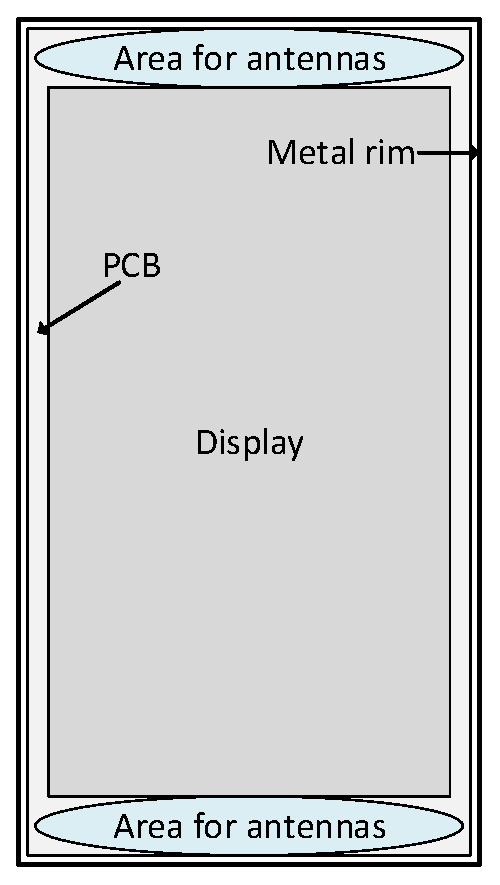
\includegraphics[width=0.9\textwidth]{img/metal_rim.eps}
        \caption{Typical locations of antennas in metal-rimmed handsets presented in \cite{ban_low_profile}.}
        \label{fig:metal_rim}
    \end{subfigure}
    \hspace{20pt}
    \begin{subfigure}[b]{0.4\textwidth}
        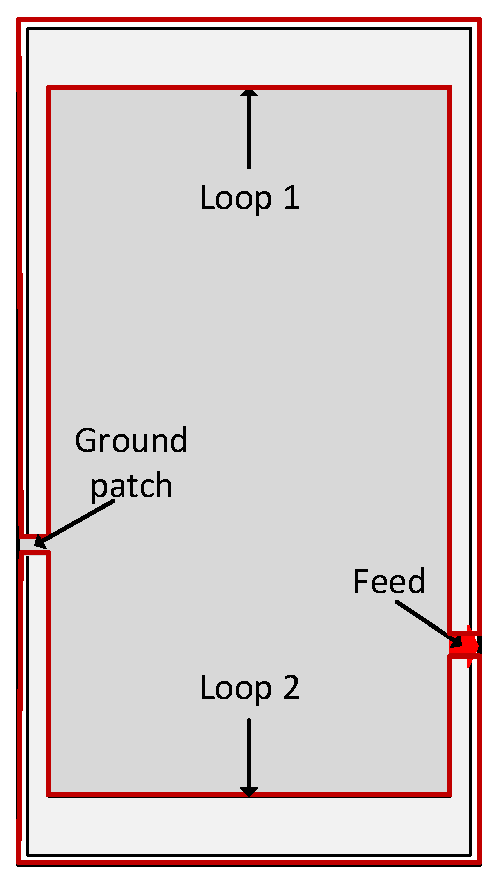
\includegraphics[width=0.9\textwidth]{img/dual_loop.eps}
        \caption{Example of a dual-loop antenna in metal-framed phone used in \cite{ban_dual_loop, stanley_lte_mimo}.}
        \label{fig:dual_loop}
    \end{subfigure}
    \caption{Proposed configurations in previous studies.}
    \label{fig:metal_rim_examples}
\end{figure}

As the display is acting as ground plane, the metal rim can be grounded with a small patch \cite{ban_dual_loop, stanley_lte_mimo}. Placing feed to another patch forms two loops between the display and the metal rim, as Figure \ref{fig:dual_loop} illustrates. This technique allows to keep the metal rim unbroken to maximize the strength of the phone. The length of the loop can be chosen such that different wave modes are excited. Since one feed-ground patch pair creates two loops of different lengths, both having own excited loop modes, this design can cover multiple frequency bands. Loops can, however, be located above the display, like traditional PIFAs \cite{reconf_narrow,hybrid}. %\cite{ban_dual_loop, stanley_lte_mimo}

Different resonant modes can be obtained also with slots in the ground plane \cite{yuan_slot}. Combining slots with loops a large number of resonance modes can be achieved \cite{hsu_compact}. Each element supports several modes that can be excited simultaneously to obtain wide bandwidth. However, slots and loops require quite large space, which is already limited. Monopole antenna in the side metal itself saves space inside the phone for other applications \cite{lee_monopole, valkonen_multifeed}. Cutting gaps to the metal rim constructs a monopole antenna, which couples with the rest of the rim to cover a wide set of frequencies \cite{chen_metal_frame}. Besides these antennas integrated into the structure, IFAs are also used \cite{hepta_ifa}. %\cite{hsu_compact, yuan_slot, lee_monopole, chen_metal_frame}

\subsection{Full metal-covered handsets}
\label{sec:full_cover}
From the metal rim on the sides of the phone, the next step is metallic back cover. Similarly to handsets with metal rim, metallic back cover improves robustness but deteriorates the performance of antennas. However, the harmful effects of full metal back cover are so strong, that many of the antenna solutions in the recent studies have slots in the cover (Figure \ref{fig:metal_covers}). In those studies antennas are either PIFAs, or monopoles or the slots themselves \cite{wu_pier, son_wideband_mimo, wu_tunable, zhong_pier}. 

Few studies have still shown promising antenna designs for handsets with full metal back cover. These designs are based on PIFAs or L-shaped strips, but they require a part of the metal rim to be removed \cite{chen_compact_lte, wu_pier}. These modifications make the handset not fully metal-covered, but as the metallic back cover is the main challenge in these cases, the proposed solutions are usable as they have achieved at least 40\,\% efficiency in the operating bands. %\cite{chen_compact_lte, wu_pier}

\begin{figure}[H]
\centering
    \begin{subfigure}[b]{0.3\textwidth}
        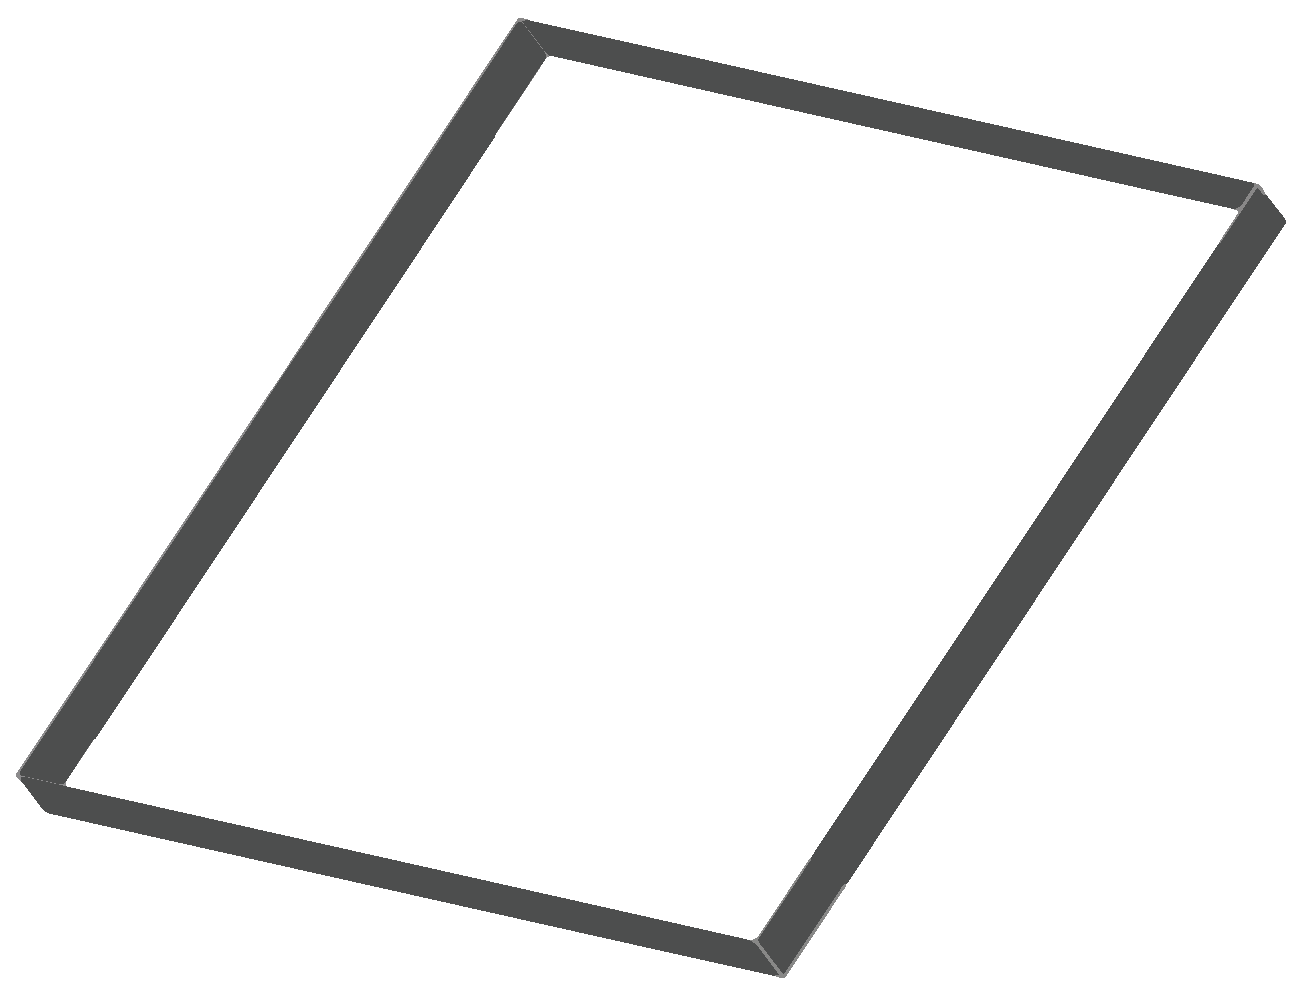
\includegraphics[width=\textwidth]{img/metal_rim2.eps}
        \caption{Metal rim.}
        \label{fig:rim}
    \end{subfigure}
    \begin{subfigure}[b]{0.3\textwidth}
        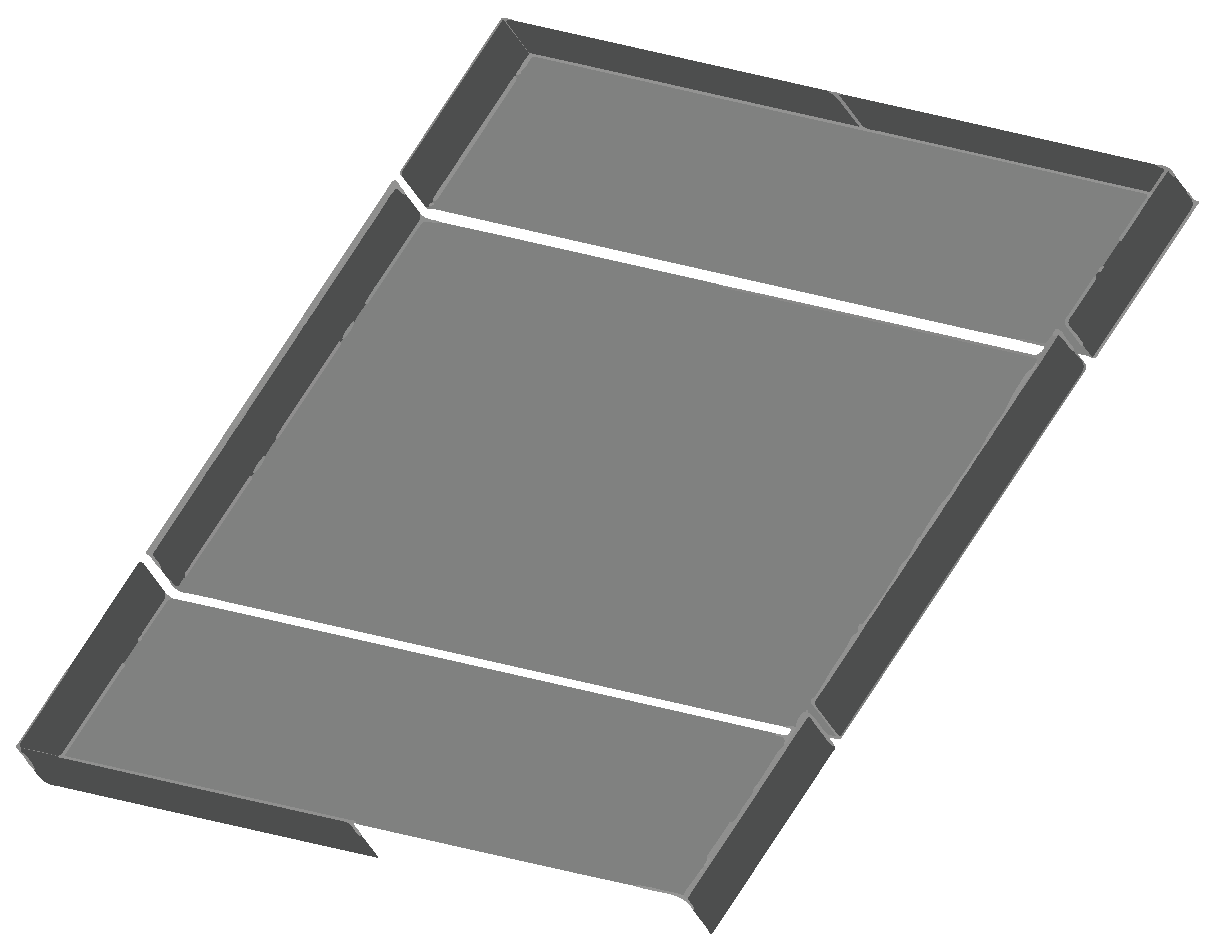
\includegraphics[width=\textwidth]{img/metal_cover_slots.eps}
        \caption{Examples of slots.}
        \label{fig:cover_slots}
    \end{subfigure}
    \begin{subfigure}[b]{0.3\textwidth}
        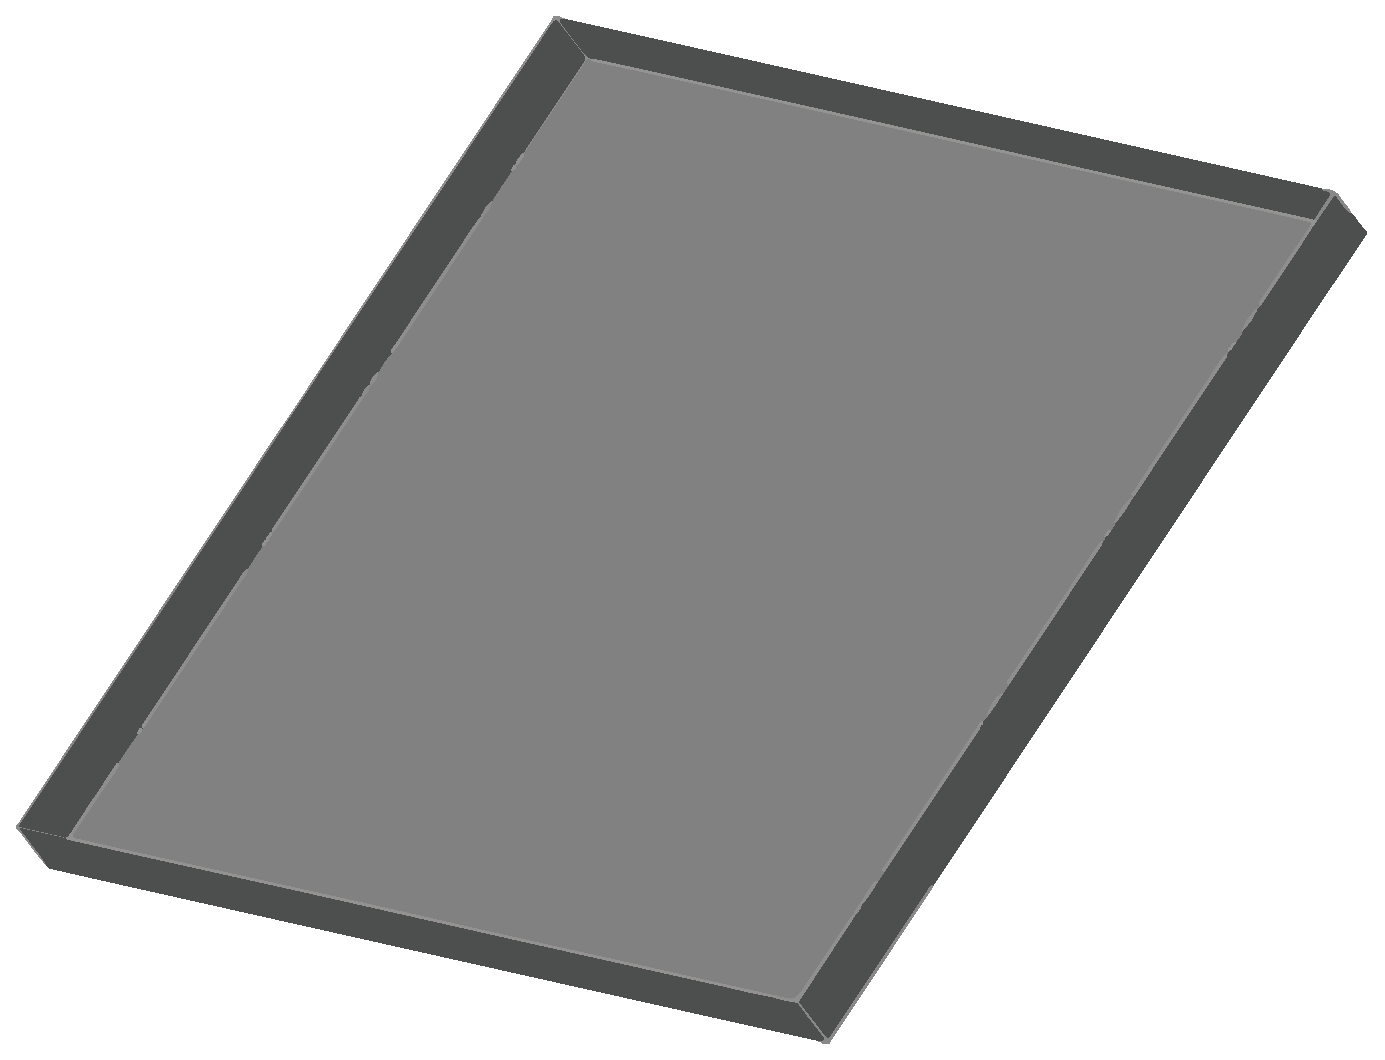
\includegraphics[width=\textwidth]{img/metal_cover_full.eps}
        \caption{Full metal cover.}
        \label{fig:full_cover}
    \end{subfigure}
    \caption{Re-illustrated examples of metal-covering of mobile phone presented in\cite{chen_compact_lte}.}
    \label{fig:metal_covers}
\end{figure}



\subsection{Key aspects in previous studies}
\label{sec:key_aspects}
More interesting matter in the previously studied antenna solutions is the technical details like operational frequencies and matching techniques, rather than positioning of antennas. As can be expected of today's mobile devices, all solutions are for LTE networks. Still, only antennas proposed in \cite{stanley_lte_mimo, son_wideband_mimo, chen_compact_lte, chen_metal_frame} support LTE bands operating at $700-800\,\mega\hertz$. These solutions tend to have average of $40\,\%$ efficiency in the low band. 

As majority of proposed solutions operate at frequencies $800-906\,\mega\hertz$ and $1.7-2.7\,\giga\hertz$, the performance of antennas in these ranges is obviously better. Typical efficiencies for lower frequencies are around $50-70\,\%$ on average and for the high band $60-80\,\%$ on average \cite{ban_dual_loop,chen_compact_lte,son_wideband_mimo,chen_metal_frame,zhong_pier}. Effect of user's hand or head is also measured in \cite{zhong_pier, chen_metal_frame,ban_dual_loop}. The effect is significant since efficiencies drop to average of $10-30\,\%$ in all supported bands. 

Handsets with metal covers and/or frames create a challenging operational environment for antennas. Besides the physical structure of an antenna, matching circuits have a major impact on final performance. Typically matching is done with lumped elements, and common amount of them is two or three for each antenna \cite{stanley_lte_mimo, zhong_pier, wu_pier}. Matching circuits improve isolation between elements leading to better element efficiency, as well as efficiency of the whole system. Even though wide band matching is desirable, it might be hard to achieve with fixed matching network. As resonance tends to occur in narrow peaks, digitally tunable capacitors (DTC) are used in antennas presented in \cite{chen_compact_lte,wu_tunable} to obtain good matching level over the whole band. To improve matching even further, few designs use band-stop \cite{lee_monopole, wu_pier} or band-pass \cite{chen_metal_frame} filters, or reactive loading \cite{chen_compact_lte, chen_metal_frame} to improve antenna's bandwidth. %\cite{stanley_lte_mimo, zhong_pier, lee_monopole, wu_pier, wu_tunable, chen_compact_lte}

The common feeding mechanism in different solutions is single-feed \cite{wu_tunable, chen_metal_frame, lee_monopole, chen_compact_lte}. That is especially for designs with one element, but also for multiple elements. Designed slot or hybrid antennas have only one feeding point, and signal couples from the fed element to the others \cite{son_wideband_mimo,hsu_compact,zhong_pier,yuan_slot}. Also dual-loop antennas presented in \cite{stanley_lte_mimo,ban_dual_loop} have just one feed for both loops. However, in that case both loops are fed. Multiple feeds are used only in designs that have also other elements than slots or loops, or have the same antenna structure copied to the other end of the phone. Clearly, in those situations each element or structure is single-fed, but total number of feeds is plural \cite{stanley_lte_mimo, son_wideband_mimo}.

In LTE networks, one way to increase bandwidth and throughput is applying MIMO techniques in data transmission. However, MIMO operations are not that much studied for metal-covered phones. First design, seen in \cite{son_wideband_mimo}, has two similar antenna structures in both ends of the phone consisting complex monopole and planar inverted F antennas. This structure provides full MIMO capability for all operating frequencies, although antennas' efficiencies are only ca. $20\,\%$ at the lowest supported frequency of $746\,\mega\hertz$. The other MIMO solution proposed in \cite{stanley_lte_mimo} has a dual-loop antenna between ground plane and side metal frame, and a capacitive coupling element (CCE) antenna. Since the CCE antenna operates only on upper frequencies ($1710-2690\,\mega\hertz$) and does not cover the lower band, the design does not have full MIMO capability. %\cite{stanley_lte_mimo, son_wideband_mimo}


\begin{sidewaystable}[H]
%\begin{table}[H]
\centering
\caption{Comparison of previously studied antennas in metal-covered phones.}
\begin{tabular}{|M{0.08\textheight}|M{0.13\textheight}|M{0.09\textheight}|M{0.15\textheight}|M{0.13\textheight}|M{0.14\textheight}|M{0.16\textheight}|}
    \hline
    \textbf{Antenna} & \textbf{Antenna type} & \textbf{Size [$\milli\meter^2$]} & \textbf{Frequencies [$\mega\hertz$]} & \textbf{Efficiency [\%]} & \textbf{Matching network} & \textbf{Metal cover style}\\
    \hline
    \cite{ban_dual_loop} & Dual-loop & $10\times70$, $5\times70$ & $824-960$, $1710-2690$ & $60-80$ & N/A & Unbroken metal rim\\
    \hline
    \cite{hsu_compact} & U-shaped loop + T-shaped slot & $64\times8$ & $791-960$, $1710-2690$, $3410-3800$ & $50-90$ & N/A & Unbroken metal rim\\
    \hline
    \cite{yuan_slot} & Slot & $56.5\times15.5$ & $824-960$, $1710-2170$ & $60-80$ & N/A & Unbroken metal rim\\
    \hline
    \cite{stanley_lte_mimo} & Dual-loop + CCE & $10\times70$, $10\times70$, $12\times6$ & $698-960$, $1710-2690$ & $50-90$ & $\Pi$-topology for both antennas & Unbroken metal rim\\
    \hline
    \cite{reconf_narrow} & & & & & & \\
    \hline
    \cite{hybrid} & & & & & & \\
    \hline
    \cite{lee_monopole} & Monopole & $50\times6.5$ & $824-960$, $1710-2690$ & $75-85$ & F-topology + band-stop filter & Metal rim\\
    \hline
    \cite{valkonen_multifeed} & & & & & & \\
    \hline
    \cite{chen_metal_frame} & Monopole & $70\times5$ & $698-960$, $1710-2690$ & $50-70$ & 4 elements + band-pass filter + reactive loading & Metal rim\\
    \hline
    \cite{hepta_ifa} & & & & & & \\
    \hline
    \cite{wu_pier} & Coupled monopoles & $20.5\times5$ & $1560-1690$, $2410-2490$, $4950-6510$ & average $40$ or $70$ & Band-stop filter & Full metal housing, with opening in the corner\\
    \hline
    \cite{son_wideband_mimo} & Monopole + IFA hybrid & $64\times16$, $64\times16$ & $746-960$, $1710-2170$, $2300-2400$ & $20-70$ & N/A & Metal back cover with slots\\
    \hline
    \cite{wu_tunable} & ILA & $35\times8$ & $824-960$, $1710-2170$ & $30-55$ & 2 elements + DTC & Full metal cover with slots\\
    \hline
    \cite{zhong_pier} & Slot & $65+20\times1$, $65\times1$, $40\times1$, $48\times1$ & $824-960$, $1560-1690$, $1710-2170$, $2410-2490$ & $40-65$ & 2 elements & Full metal cover with slots\\
    \hline
    \cite{chen_compact_lte} & Loop & $64\times8$ & $700-960$, $1710-2170$ & average $45$ or $60$ & 3 elements + 2 DTCs & Full metal housing with opening at the end of the phone\\
    \hline
\end{tabular}
%\end{table}
\end{sidewaystable}

\clearpage